\documentclass[10pt,twocolumn,letterpaper]{article}

% ---------- Codificación e idioma ----------
\usepackage[utf8]{inputenc}
\usepackage[T1]{fontenc}
\usepackage{mathptmx}
\usepackage[spanish,es-nodecimaldot,es-tabla,es-noquoting]{babel}

% ---------- Formato ----------
\usepackage[top=2cm,bottom=2cm,left=1.8cm,right=1.8cm,columnsep=0.7cm]{geometry}
\usepackage{microtype}
\usepackage{setspace}
\usepackage{enumitem}
\usepackage{booktabs}
\usepackage{tabularx}
\usepackage{array}
\usepackage{graphicx}
\usepackage{xcolor}
\usepackage{caption}
\usepackage{titlesec}
\titleformat{\section}{\large\bfseries}{\thesection.}{0.5em}{}
\titlespacing*{\section}{0pt}{7pt}{2pt}
\titleformat{\subsection}{\normalsize\bfseries}{\thesubsection.}{0.5em}{}
\titlespacing*{\subsection}{0pt}{5pt}{2pt}
\usepackage[hidelinks]{hyperref}

% ---------- Matemáticas ----------
\usepackage{amsmath,amssymb}

% ---------- Algoritmo ----------
\usepackage{algorithm}
\usepackage{algpseudocode}
\floatname{algorithm}{Algoritmo}
\renewcommand{\algorithmicfor}{\textbf{PARA}}
\renewcommand{\algorithmicforall}{\textbf{PARA CADA}}
\renewcommand{\algorithmicdo}{\textbf{HACER}}
\renewcommand{\algorithmicif}{\textbf{SI}}
\renewcommand{\algorithmicthen}{\textbf{ENTONCES}}
\renewcommand{\algorithmicelse}{\textbf{SINO}}
\renewcommand{\algorithmicend}{\textbf{FIN}}
\renewcommand{\algorithmicwhile}{\textbf{MIENTRAS}}
\renewcommand{\algorithmicreturn}{\textbf{DEVOLVER}}
\renewcommand{\algorithmicfunction}{\textbf{FUNCIÓN}}

% ---------- Citas autor-año ----------
\usepackage[round,authoryear]{natbib}

\setlength{\parindent}{0pt}
\setlength{\parskip}{3pt}
\setlist{itemsep=0pt,topsep=2pt,parsep=0pt}
\captionsetup{font=small,labelfont=bf}

% ---------- Macros ----------
\newcommand{\R}{\mathbb{R}}
\newcommand{\AUC}{\mathrm{AUC}}

% =====================================================
\title{\vspace{-1.2cm}\Large\bfseries Búsqueda Evolutiva de Funciones de Activación mediante Programación Genética Lineal Epigenética: Observaciones sobre Diversidad de Datos, Comparación Estadística y Transferencia Geotérmica}
\author{
    \large Rubén Rivera García \\
    \normalsize Centro de Investigación Científica y de Educación Superior de Ensenada (CICESE) \\
    \normalsize Maestría en Ciencias en Ciencias de la Computación \\
    \normalsize Curso: Inteligencia Computacional para Optimización (ICO 2026-3) \\
    \normalsize Instructor: Dr.\ Jesús Guillermo Falcón-Cardona
}
\date{}

\begin{document}

\maketitle

% =====================================================
\section*{RESUMEN}
Este trabajo investiga la síntesis evolutiva de funciones de activación en redes neuronales profundas mediante Programación Genética Lineal Epigenética (ELGP). Se formuló un problema mono-objetivo con restricciones basado en la aptitud normalizada agregada ($\bar{z}$) respecto a una red base ReLU sobre múltiples conjuntos de datos, resuelto mediante una estrategia $(\mu=30, \lambda=60)$ con reglas de Deb y archivo élite. Con $N=10$ conjuntos de entrenamiento (2{,}647 evaluaciones efectivas, $\approx 44$ generaciones en el clúster Ixachi), el algoritmo convergió a una transformación afín de LeakyReLU ($\alpha \approx 0.248$, simplificada a $\alpha = 0.25$, $r = 1.0000$), donde la razón de pendientes emerge de $e_k = 0.7524$ sobre $\max(0, v)$ bajo una restricción de no linealidad que acota analíticamente $\alpha \lesssim 0.37$. La comparación con exploraciones previas ($N=1, 5$) ilustra una transición desde perfiles cuasi-lineales hacia modelos lineales por tramos, modulada por la diversidad del banco de entrenamiento. En 5 conjuntos de prueba disjuntos, ELGP quedó entre $-0.0031$ y $-0.0006$ AUC frente a los baselines no lineales modernos; con $n=5$ conjuntos los intervalos de confianza no descartan diferencias de $\approx 0.013$ ni distinguen una red lineal ($p_{\mathrm{crudo}}=0.1097$, $p_{\mathrm{Holm}}=1.0000$), arrojando resultados inconclusos más que evidencia de equivalencia. Los controles pareados evidenciaron degradación generalizada en reevaluación multisemilla, consistente con sesgo de selección y sobreajuste a la exploración. Finalmente, en la transferencia a susceptibilidad geotérmica en Baja California (29.35M píxeles), se demuestra algebraicamente que BatchNorm absorbe escala y traslación; las discrepancias cartográficas son compatibles con la varianza estocástica de semilla única, mientras que el AUC en prueba ($>0.999$) refleja la influencia de la fuga espacial en un esquema positivo-no etiquetado.

\vspace{0.3em}
\hrule
\vspace{0.4em}

% =====================================================
\section{INTRODUCCIÓN}

La elección de la función de activación $\varphi:\R\to\R$ define la dinámica del gradiente y la capacidad representacional en redes neuronales profundas. Si bien la práctica común descansa en funciones estándar como ReLU \citep{nair2010}, GELU \citep{hendrycks2016} o Swish \citep{ramachandran2018}, el diseño algorítmico automatizado mediante cómputo evolutivo permite explorar el espacio de operadores continuos de manera sistemática \citep{real2020automl,bingham2020}.

Este estudio se enfoca en dos aspectos centrales:
\begin{enumerate}[leftmargin=1.2em]
  \item \textbf{Diversidad y estructura matemática:} Observar cómo varía la forma de la función descubierta al ejecutar la búsqueda sobre un único conjunto de datos frente a bancos de $N=5$ y $N=10$ conjuntos de datos bajo sus respectivas formulaciones de restricción.
  \item \textbf{Evaluación y transferencia:} Medir si la activación resultante muestra ventajas en conjuntos de datos no vistos y analizar críticamente su comportamiento al transferirse a la cartografía de susceptibilidad geotérmica regional.
\end{enumerate}

% =====================================================
\section{MÉTODO Y FORMULACIÓN MATEMÁTICA}

\textbf{Representación cromosómica.} Cada individuo se codifica como un programa lineal de $L=8$ instrucciones sobre registros $\{r_0, r_1, r_2\}$. La señal de entrada $v$ se carga en $r_0$ y el resultado se lee del mismo registro. El repertorio de operadores comprende:
\begin{align}
  \mathcal{F} = \{&+, \times, \mathrm{pdiv}, \max, \sin, \cos, \sigma, \tanh, \mathrm{ReLU}, \nonumber \\
  &\mathrm{leaky\_relu}, \mathrm{gelu}, \mathrm{elu}, \mathrm{selu}, \mathrm{softplus}, \mathrm{swish}, v^2, e^{-v^2}\},
\end{align}
donde $\mathrm{pdiv}(a, b) = a / (b + \mathrm{sgn}(b)\cdot 10^{-5})$ es una división protegida, y $\mathrm{leaky\_relu}$ cuenta con pendiente negativa fija $\alpha = 0.10$. Dado que $\mathrm{ReLU}$, $\mathrm{leaky\_relu}$ y $\max$ forman parte de $\mathcal{F}$, la emergencia de perfiles lineales por tramos constituye una recombinación de bloques provistos en el conjunto de primitivas.

Cada instrucción $k$ incluye un peso continuo epigenético $e_k \in [0, 1]$ que modula la actualización del registro destino:
\begin{equation}
  r_{\mathrm{dest}} \leftarrow (1 - e_k)\, r_{\mathrm{dest}} + e_k \cdot \mathrm{op}(r_{\mathrm{src1}}, r_{\mathrm{src2}}).
\end{equation}

\textbf{Optimización mono-objetivo con restricciones.} El problema se formula como la minimización de la puntuación estandarizada agregada con una restricción de no linealidad mínima. Para cada conjunto de datos de entrenamiento $j \in \{1, \dots, M\}$, se calibra previamente la media $\mu_j$ y la desviación estándar $\sigma_j$ del $\AUC$ (Macro One-vs-Rest en multiclase) de una red base con ReLU sobre $K=3$ pliegues.

La aptitud de un individuo $\mathbf{x}$ corresponde a la media de puntuaciones estandarizadas:
\begin{equation}
  \bar{z}(\mathbf{x}) = \frac{1}{M}\sum_{j=1}^M \frac{\AUC_j(\mathbf{x}) - \mu_j}{\sigma_j}.
\end{equation}
El problema se define como:
\begin{equation}
  \min_{\mathbf{x}} f(\mathbf{x}) = -\bar{z}(\mathbf{x}) \quad \text{s.a.} \quad g_1(\mathbf{x}) = \epsilon_{\mathrm{nl}} - \mathrm{NL}(\mathbf{x}) \le 0,
\end{equation}
donde $\mathrm{NL}(\mathbf{x}) = 1 - R^2$ proviene de la regresión lineal de $\varphi_{\mathbf{x}}(v)$ contra $v$ sobre una malla de 200 puntos uniformes en $[-3, 3]$ \citep{leshno1993}, con umbral $\epsilon_{\mathrm{nl}} = 0.05$. Si la función genera valores no finitos o es constante, se asigna $g_1 = 1.0$.

\textbf{Efecto analítico de la restricción $g_1$:} Para una función LeakyReLU con pendiente negativa relativa $\alpha \in [0, 1]$ evaluada en $[-L, L]$ (invariante ante transformaciones afines con escala positiva), la no linealidad analítica continua es:
\begin{equation}
  \mathrm{NL}(\alpha) = \frac{(1-\alpha)^2}{5 + 6\alpha + 5\alpha^2}.
\end{equation}
Para $\alpha = 0.25$, se tiene $\mathrm{NL}(0.25) \approx 0.0826$ en teoría continua ($0.0831$ en la discretización de 200 puntos). La condición de factibilidad $\mathrm{NL}(\alpha) \ge 0.05$ impone analíticamente $\alpha \lesssim 0.371$. Por consiguiente, la restricción $g_1$ en $N=10$ fuerza la presencia de un quiebre angular marcado, descartando funciones cuasi-lineales ($\alpha > 0.37$). En contraste, las exploraciones previas con $N=1$ y $N=5$ emplearon una restricción de varianza mínima $\epsilon_v - \mathrm{Var}(\varphi(V)) \le 0$ ($\epsilon_v = 10^{-4}$), la cual permitía fenotipos casi lineales.

\textbf{Estrategia evolutiva y operadores.} Se implementó una estrategia evolutiva $(\mu, \lambda)$ con $\mu=30$ padres y $\lambda=60$ descendientes por generación ($\approx 44$ generaciones para 2{,}647 evaluaciones efectivas), con selección generacional por coma combinada con un archivo externo élite. En la selección por torneo ($k=3$) se aplican las reglas de Deb \citep{deb2000}.

Los operadores corresponden a cruza uniforme ($P_{\mathrm{cross}} = 1.0$) y mutación estructural por instrucción ($p_m = 0.20$), acompañada de perturbación gaussiana $\mathcal{N}(0, 0.1^2)$ en $e_k$, acotada en $[0, 1]$. Cada candidato se evaluó entrenando un MLP de 3 capas ocultas (64 unidades, BatchNorm) durante un máximo de 40 épocas con Adam ($\mathrm{lr}=0.002$, tamaño de lote 256) y parada temprana con paciencia de 6 épocas evaluada sobre una reserva interna del 15\%. Se define una \textbf{evaluación efectiva} como un entrenamiento completo que requirió cálculo de red, omitiendo individuos descartados por el filtro rápido y consultas cacheadas. El procedimiento evolutivo se resume en el Algoritmo~\ref{alg:elgp}.

\begin{algorithm}[t]
\caption{Búsqueda Evolutiva ELGP-Activación}
\label{alg:elgp}
\scriptsize
\begin{algorithmic}[1]
\Function{evaluar}{$\mathbf{x}$} \Comment{Aptitud del candidato $\mathbf{x}$}
  \State $g_1 \leftarrow \epsilon_{\mathrm{nl}} - \mathrm{NL}(\mathbf{x})$
  \If{$g_1 > 0$ \textbf{o} $\varphi_{\mathbf{x}}$ diverge} \Comment{Filtro rápido (Fast-Fail)}
    \State \Return $(+\infty, g_1)$ \Comment{Descarta entrenamiento sin cómputo}
  \EndIf
  \State $Z \leftarrow [\,]$
  \For{$j \in \{1, \dots, M\}$} \Comment{$M=10$ conjuntos, $K=3$ pliegues}
    \State $\AUC_j \leftarrow \text{entrenar\_y\_validar}(\varphi_{\mathbf{x}}, \mathcal{D}_j)$
    \If{$\AUC_j$ no es finito}
      \State \Return $(+\infty, 1.0)$ \Comment{Divergencia numérica}
    \EndIf
    \State $Z.\text{agregar}((\AUC_j - \mu_j) / \sigma_j)$
  \EndFor
  \State \Return $(f = -\mathrm{promedio}(Z),\, 0)$ \Comment{Minimizar $-\bar{z}$}
\EndFunction
\Statex
\Function{hijos}{$\mathcal{P}$, $\text{estancamiento}$}
  \State $\mathcal{H} \leftarrow [\,]$
  \While{$|\mathcal{H}| < \lambda$} \Comment{$\lambda = 60$ descendientes}
    \State $\mathbf{p}_1, \mathbf{p}_2 \leftarrow \text{torneo}(\mathcal{P}, k=3)$ \Comment{Reglas de factibilidad de Deb}
    \State $\mathcal{H}.\text{agregar}(\text{mutar}(\text{cruza}(\mathbf{p}_1, \mathbf{p}_2, 1.0)))$
  \EndWhile
  \If{$\text{estancamiento} \ge 5$} \Comment{Control anti-estancamiento}
    \State $\mathcal{H}[45:] \leftarrow 15 \text{ individuos factibles al azar}$
  \EndIf
  \State \Return $\mathcal{H}$
\EndFunction
\Statex
\State \textbf{Procedimiento principal:}
\State $\mathcal{P} \leftarrow 30 \text{ individuos factibles al azar}$; $\mathcal{E} \leftarrow \emptyset$ \Comment{Archivo élite}
\ForAll{$\mathbf{x} \in \mathcal{P}$}
  \State $(f(\mathbf{x}), g_1(\mathbf{x})) \leftarrow \Call{evaluar}{\mathbf{x}}$
\EndFor
\State $\mathcal{E} \leftarrow \text{actualizar\_élites}(\mathcal{E}, \mathcal{P})$
\State $f_{\mathrm{campeón}} \leftarrow \min_{\mathbf{x} \in \mathcal{P}} f(\mathbf{x})$; $\text{estancamiento} \leftarrow 0$
\For{$\text{gen} \in \{1, \dots, G_{\max}\}$} \Comment{$G_{\max} \approx 44$ generaciones}
  \State $\mathcal{H} \leftarrow \Call{hijos}{\mathcal{P}, \text{estancamiento}}$
  \ForAll{$\mathbf{x} \in \mathcal{H}$ con $\mathbf{x} \notin \mathcal{E}$}
    \State $(f(\mathbf{x}), g_1(\mathbf{x})) \leftarrow \Call{evaluar}{\mathbf{x}}$
  \EndFor
  \State $\mathcal{P} \leftarrow \text{selección}(\mathcal{H}, \mu=30)$ \Comment{Estrategia generacional $(\mu, \lambda)$}
  \State $\mathcal{E} \leftarrow \text{actualizar\_élites}(\mathcal{E}, \mathcal{P})$
  \If{$\min_{\mathbf{x} \in \mathcal{P}} f(\mathbf{x}) < f_{\mathrm{campeón}}$}
    \State $f_{\mathrm{campeón}} \leftarrow \min_{\mathbf{x} \in \mathcal{P}} f(\mathbf{x})$; $\text{estancamiento} \leftarrow 0$
  \Else
    \State $\text{estancamiento} \leftarrow \text{estancamiento} + 1$
  \EndIf
\EndFor
\State \Return $\mathcal{E}$
\end{algorithmic}
\end{algorithm}

% =====================================================
\section{EXPERIMENTACIÓN Y RESULTADOS EN HPC}

\subsection{Infraestructura, Tiempos y Suite de Datos}
La experimentación se ejecutó en un nodo Intel Xeon Gold 5320 (32 GB RAM) del clúster Ixachi de CICESE. El trabajo completo para $N=10$ conjuntos de datos (Job 21128) requirió 2{,}468.2 minutos (41.13 horas):
\begin{enumerate}[leftmargin=1.2em]
  \item \textbf{Calibración baseline:} Estimación de $\mu_j, \sigma_j$ para ReLU en los 10 conjuntos de búsqueda ($\approx 2$ min).
  \item \textbf{Búsqueda ELGP:} 2{,}647 evaluaciones efectivas (703.8 min / 11.7 h, 44 generaciones).
  \item \textbf{Controles pareados:} Búsqueda Aleatoria (2{,}647 evals, 703.0 min / 11.7 h) y Ablación $e_k=1$ fijo (2{,}647 evals, 736.5 min / 12.3 h).
  \item \textbf{Evaluación exhaustiva final:} 16 métodos sobre 19 conjuntos de datos con 10 semillas y 5 pliegues ($\approx 325$ min).
\end{enumerate}

Las exploraciones con $N=1$ y $N=5$ corresponden a corridas previas independientes ejecutadas bajo la misma arquitectura de hardware.

Se evaluaron 19 conjuntos de datos de UCI Machine Learning Repository:
\begin{itemize}[leftmargin=1.2em]
  \item \textbf{Búsqueda evolutiva ($N=10$):} Credit Card ($n=30{,}000$), German Credit ($n=1{,}000$), Wine Quality ($n=6{,}497$), Magic Gamma ($n=19{,}020$), Vehicle ($n=846$), Spambase ($n=4{,}601$), Bank Marketing ($n=45{,}211$), Australian Credit ($n=690$), Raisin ($n=900$) y Obesity ($n=2{,}111$). Para conjuntos con $n > 10{,}000$, se utilizó una submuestra estratificada de 4{,}000 instancias durante la búsqueda.
  \item \textbf{Generalización no vista ($N=5$):} Steel Plates ($n=1{,}941$), Yeast ($n=1{,}484$), Sonar ($n=208$), Heart Disease ($n=303$) y Blood Transfusion ($n=748$).
  \item \textbf{Chequeo de cordura ($N=4$):} Datasets saturados con $\AUC \ge 0.985$ (Statlog Landsat, Dry Bean, Digits, Breast Cancer), evaluados para verificar estabilidad y excluidos a posteriori de los contrastes estadísticos para evitar efectos de techo.
\end{itemize}

\subsection{Evolución Morfológica según la Diversidad ($N$)}
Las expresiones analíticas descubiertas muestran el siguiente patrón:
\begin{itemize}[leftmargin=1.2em]
  \item \textbf{$N = 1$ dataset (Credit Card):} Bajo la restricción de varianza previa, emergió $\varphi(v) \approx 0.62 v + 0.38 \sin(0.45 \sigma(v))$. Como $\sigma(v) \in (0, 1)$, el argumento satisface $0.45 \sigma(v) \in (0, 0.45)$. Mediante aproximación de Taylor, $|x - \sin x| \le x^3 / 6 \approx 0.0152$ para $x=0.45$; multiplicado por $0.38$, el error máximo al linealizar el operador seno externo es de $\approx 0.0058$, reduciendo la expresión a $\varphi(v) \approx 0.62 v + 0.171 \sigma(v)$. Dado que el término lineal $0.62v$ domina en amplitud a $0.171\sigma(v)$ sobre $[-3, 3]$, la función resultante es cuasi-lineal ($\mathrm{NL} = 1 - R^2 \approx 4\times 10^{-5}$, infactible bajo el $g_1$ posterior de $N=10$). Planteamos como hipótesis que esto responde a la estructura del problema: una regresión logística simple en Credit Card alcanza $\AUC = 0.7227 \pm 0.0039$, mientras que el baseline de ReLU calibrado en la misma submuestra obtuvo $0.7336 \pm 0.0113$. Esta cercanía competitiva de modelos lineales indujo una función cuasi-lineal, la cual no aportó ventaja representacional al transferirse fuera de Credit Card frente a modelos lineales estándar.
  \item \textbf{$N = 5$ datasets:} Al agregar dominios diversos bajo la misma restricción de varianza, la búsqueda se orientó hacia linealidad por tramos: $\varphi(v) = 0.19 u + 0.81 \mathrm{relu}(u)$ con $u = 0.50 v + 0.50 \sin(0.33\,\mathrm{gelu}(v))$, aproximando a LeakyReLU con $\alpha \approx 0.146$ ($r = 0.9999$). Dado que la transición $N=1 \to 5$ ocurrió sin cambiar la restricción, el enriquecimiento funcional estuvo guiado directamente por la diversidad de datos.
  \item \textbf{$N = 10$ datasets:} La búsqueda convergió analíticamente a:
  \begin{equation}
    \varphi(v) = 0.85\,\bigl(0.25\,v + 0.75\,\max(0, v)\bigr) + 0.15.
  \end{equation}
\end{itemize}

Para $v > 0$, la pendiente es $m_+ = 0.8500$; para $v \le 0$, es $m_- = 0.85 \times 0.25 = 0.2125$, lo que define una transformación afín de LeakyReLU con pendiente negativa relativa $\alpha = m_- / m_+ = 0.25$. La inspección del genoma muestra que la instrucción determinante fue $r_0 \leftarrow (1 - e_k)r_0 + e_k \max(r_2, r_0)$ con $r_2=0$ y $e_k = 0.7524$, de modo que la razón de pendientes $\alpha = 1 - e_k \approx 0.2476$ (redondeada analíticamente a $0.25$, $r=1.0000$) emerge del ajuste continuo del peso epigenético sobre el bloque $\max(0, v)$.

\begin{figure}[t]
\centering
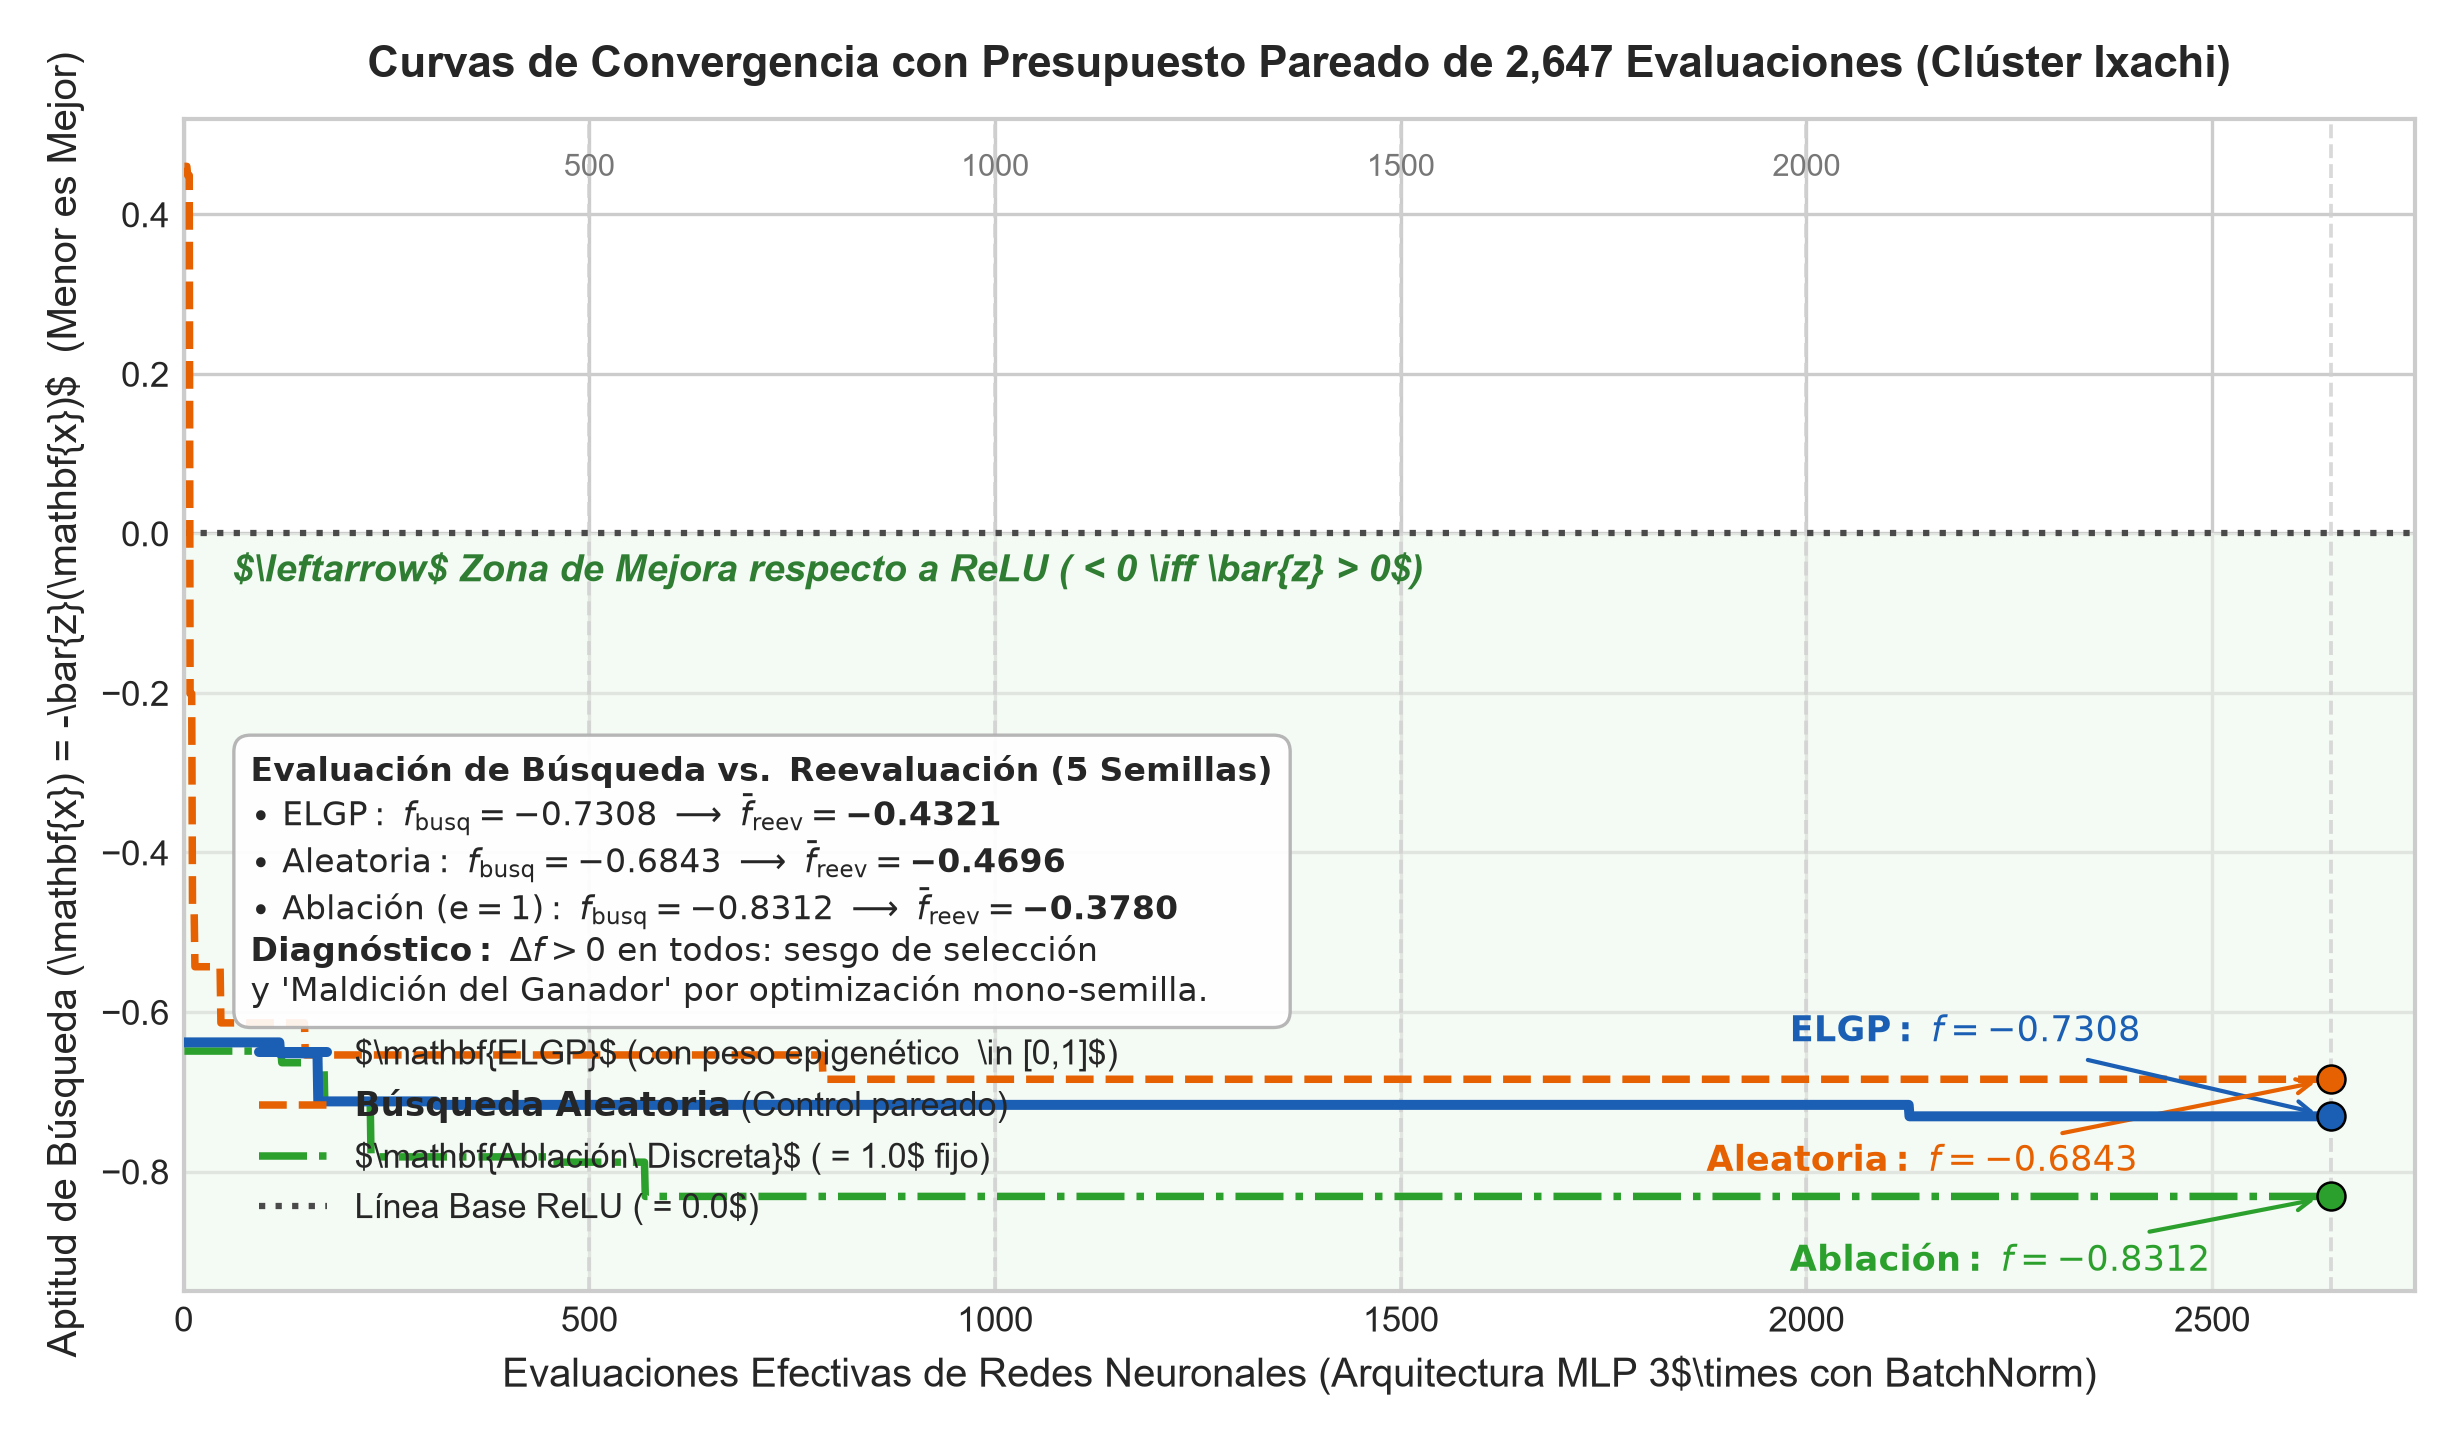
\includegraphics[width=\columnwidth]{convergencia_comparativa.png}
\caption{Curvas de convergencia bajo presupuesto pareado de 2{,}647 evaluaciones ($f = -\bar{z}$; menor es mejor).}
\label{fig:convergencia}
\end{figure}

\subsection{Comportamiento de Controles y Desglose de Aptitud}
La Figura~\ref{fig:convergencia} ilustra la convergencia de mejor aptitud histórica:
\begin{itemize}[leftmargin=1.2em]
  \item \textbf{Búsqueda Aleatoria:} Registró $f = -0.6843$ en búsqueda y promedió $f = -0.4696$ en la reevaluación multisemilla (5 semillas).
  \item \textbf{ELGP:} Alcanzó $f = -0.7308$ en búsqueda y $f = -0.4321$ en reevaluación multisemilla.
  \item \textbf{Ablación ($e_k = 1.0$):} Alcanzó $f = -0.8312$ en búsqueda y descendió a $f = -0.3780$ en reevaluación multisemilla.
\end{itemize}

Los tres métodos experimentaron una pérdida sustancial de aptitud entre la fase de búsqueda y la reevaluación multisemilla, comportamiento consistente con sobreajuste a la semilla única utilizada en la exploración y sesgo de selección (maldición del ganador). En la reevaluación, la Búsqueda Aleatoria obtuvo un valor ligeramente superior en magnitud a ELGP ($-0.4696$ frente a $-0.4321$). La ablación con $e_k=1$ fijo restringe la capacidad expresiva al impedir sintonizar pendientes intermedias continuas ($\alpha = 1 - e_k$).

\begin{table}[!htbp]
\centering
\footnotesize
\setlength{\tabcolsep}{2.5pt}
\caption{Desglose de aptitud reevaluada de ELGP ($f=-0.4321$, 5 semillas) en los 10 datasets de búsqueda ($K=3$). Se indica el tamaño total ($n_{\mathrm{tot}}$) y el evaluado en búsqueda ($n_{\mathrm{busq}}$).}
\label{tab:desglose_z}
\begin{tabularx}{\columnwidth}{@{}>{\raggedright\arraybackslash}Xccccr@{}}
\toprule
Dataset & $n_{\mathrm{tot}}$ & $n_{\mathrm{busq}}$ & $\mu_{\mathrm{ReLU}}$ & $\sigma_{\mathrm{ReLU}}$ & $z_j$ (ELGP) \\
\midrule
Credit Card       & 30{,}000 & 4{,}000 & 0.7336 & 0.0113 & $+0.1071$ \\
German Credit     & 1{,}000  & 1{,}000 & 0.7653 & 0.0309 & $+0.0988$ \\
Wine Quality      & 6{,}497  & 6{,}497 & 0.8262 & 0.0108 & $+0.0223$ \\
Magic Gamma       & 19{,}020 & 4{,}000 & 0.9060 & 0.0077 & $+0.2565$ \\
Vehicle (4 cl)    & 846      & 846     & 0.9422 & 0.0063 & $\mathbf{+1.3125}$ \\
Spambase          & 4{,}601  & 4{,}601 & 0.9795 & 0.0057 & $+0.1483$ \\
Bank Marketing    & 45{,}211 & 4{,}000 & 0.8686 & 0.0071 & $+0.6825$ \\
Australian Credit & 690      & 690     & 0.9116 & 0.0328 & $+0.3315$ \\
Raisin            & 900      & 900     & 0.9252 & 0.0225 & $+0.0421$ \\
Obesity (7 cl)    & 2{,}111  & 2{,}111 & 0.9825 & 0.0025 & $\mathbf{+1.3196}$ \\
\midrule
\multicolumn{5}{@{}l}{\textbf{Promedio ($\bar{z}$)}} & $\mathbf{+0.4321}$ \\
\bottomrule
\end{tabularx}
\end{table}

La Tabla~\ref{tab:desglose_z} desglosa las puntuaciones $z_j$. Debe notarse que la estimación de $\sigma_j$ a partir de solo $K=3$ pliegues conlleva un error relativo intrínseco de $\approx 50\%$, volviendo a la métrica agregada $\bar{z}$ sensible al ruido de escala. Dos problemas multiclase pequeños, \emph{Vehicle} ($z = +1.3125$) y \emph{Obesity} ($z = +1.3196$), aportan más del 60\% de $\bar{z}$. En Obesity, su inclusión en búsqueda contrasta con la exclusión posterior de otros conjuntos saturados ($\AUC \ge 0.985$), pesando un 30.5\% de la aptitud debido a su ínfimo $\sigma_j = 0.0025$.

Asimismo, mientras que en la búsqueda con submuestras y $K=3$ pliegues se obtuvo $\bar{z}=+0.4321$ ($\sum z_j \sigma_j / 10 \approx +0.0036$ de AUC nominal), en la evaluación final con datos completos, 10 semillas y 5 pliegues, la diferencia media ELGP $-$ ReLU en estos 10 datasets se contrajo a $+0.0008$ ($0.9008$ vs $0.9000$). De hecho, la primitiva $\mathrm{leaky\_relu}$ ($\alpha=0.10$) ya presente en $\mathcal{F}$ igualó a ELGP ($0.9010$ vs $0.9008$). Además, las ganancias aparentes en multiclase no se replicaron en los conjuntos multiclase no vistos (Yeast $+0.0014$, Steel $-0.0013$).

\subsection{Evaluación en Datasets No Vistos}
Se evaluaron 16 métodos sobre 5 conjuntos disjuntos de UCI mediante 10 semillas y 5 pliegues (50 realizaciones por conjunto). La Tabla~\ref{tab:generalizacion} presenta los valores medios de AUC (Macro-OvR).

\begin{table}[!htbp]
\centering
\footnotesize
\setlength{\tabcolsep}{3pt}
\caption{Evaluación en datasets no vistos de generalización (AUC medio Macro-OvR, 10 semillas $\times$ 5 pliegues). Muestra de 9 de los 16 métodos evaluados.}
\label{tab:generalizacion}
\begin{tabularx}{\columnwidth}{@{}>{\raggedright\arraybackslash}Xccccc@{}}
\toprule
Activación & Yeast & Steel & Sonar & Heart & Blood \\
\midrule
\textbf{ELGP (10ds)} & 0.8635 & 0.9454 & 0.8846 & 0.8983 & 0.7532 \\
LeakyReLU (0.25)     & 0.8615 & 0.9460 & 0.8897 & 0.8985 & 0.7527 \\
ReLU                 & 0.8621 & 0.9467 & 0.9041 & 0.8917 & 0.7458 \\
GELU                 & 0.8594 & 0.9454 & 0.8988 & 0.8935 & 0.7561 \\
Swish                & 0.8606 & 0.9441 & 0.8916 & 0.8986 & 0.7591 \\
Tanh                 & 0.8444 & 0.9446 & 0.8628 & 0.9047 & 0.7578 \\
Sigmoid              & 0.8469 & 0.9434 & 0.8580 & 0.9031 & 0.7562 \\
Aleatoria            & 0.8456 & 0.9439 & 0.8922 & 0.8965 & 0.7545 \\
Ablación ($e=1$)     & 0.8515 & 0.9433 & 0.8894 & 0.8967 & 0.7565 \\
\bottomrule
\end{tabularx}
\end{table}

\textbf{Inferencia estadística pareada:} Se aplicó una prueba $t$ pareada sobre los 5 datasets de generalización ($\Delta = \mathrm{AUC}(\mathrm{ELGP}) - \mathrm{AUC}(\mathrm{m\acute{e}todo})$, 4 g.l.) con ajuste secuencial de \citet{holm1979} para las 15 comparaciones frente a ELGP. Se incluyeron baselines canónicos y avanzados: PReLU \citep{he2015prelu}, Mish \citep{misra2019mish}, ELU \citep{clevert2016elu} y SELU \citep{klambauer2017selu}. Cabe señalar que \citet{demsar2006} desaconseja pruebas $t$ pareadas sobre pocos conjuntos de datos y recomienda contrastes no paramétricos (Wilcoxon o Friedman).

\begin{table}[!htbp]
\centering
\footnotesize
\setlength{\tabcolsep}{3.5pt}
\caption{Comparación pareada frente a ELGP sobre los 5 datasets de generalización ($\Delta = \text{ELGP} - \text{método}$, prueba $t$ pareada, 4 g.l.). En todas las comparaciones se obtuvo $p_{\mathrm{Holm}} = 1.0000$.}
\label{tab:estadistica}
\begin{tabularx}{\columnwidth}{@{}>{\raggedright\arraybackslash}Xccc@{}}
\toprule
Comparación & Dif. ($\Delta$) & IC 95\% & $p_{\mathrm{crudo}}$ \\
\midrule
vs ReLU             & $-0.0011$ & $[-0.0146, +0.0125]$ & 0.8352 \\
vs LeakyReLU 0.25   & $-0.0007$ & $[-0.0040, +0.0026]$ & 0.6005 \\
vs LeakyReLU 0.10   & $-0.0031$ & $[-0.0158, +0.0095]$ & 0.5302 \\
vs LeakyReLU 0.01   & $-0.0011$ & $[-0.0125, +0.0103]$ & 0.8214 \\
vs PReLU            & $-0.0006$ & $[-0.0051, +0.0038]$ & 0.7118 \\
vs GELU             & $-0.0016$ & $[-0.0112, +0.0079]$ & 0.6605 \\
vs Swish            & $-0.0018$ & $[-0.0073, +0.0036]$ & 0.4102 \\
vs Mish             & $-0.0021$ & $[-0.0069, +0.0026]$ & 0.2784 \\
vs ELU              & $+0.0018$ & $[-0.0069, +0.0106]$ & 0.5942 \\
vs SELU             & $+0.0060$ & $[-0.0083, +0.0202]$ & 0.3100 \\
vs Tanh             & $+0.0062$ & $[-0.0104, +0.0228]$ & 0.3598 \\
vs Sigmoid          & $+0.0075$ & $[-0.0094, +0.0244]$ & 0.2837 \\
vs Aleatoria        & $+0.0025$ & $[-0.0092, +0.0141]$ & 0.5905 \\
vs Ablación ($e=1$) & $+0.0015$ & $[-0.0066, +0.0097]$ & 0.6304 \\
vs Lineal           & $+0.0170$ & $[-0.0060, +0.0399]$ & 0.1097 \\
\bottomrule
\end{tabularx}
\end{table}

Frente a ReLU, LeakyReLU, PReLU, GELU, Swish y Mish, ELGP quedó entre $-0.0031$ y $-0.0006$ AUC en promedio. No obstante, con $n=5$ conjuntos los intervalos de confianza (p.\,ej. $[-0.0146, +0.0125]$ frente a ReLU) no descartan diferencias de $\approx 0.013$ AUC, y el contraste tampoco distingue una red lineal sin activación ($+0.0170$, $p_{\mathrm{crudo}}=0.1097$). Los resultados son estadísticamente inconclusos y no constituyen evidencia formal de equivalencia. Asimismo, aunque ELGP y LeakyReLU(0.25) son funcionalmente equivalentes bajo BatchNorm, difieren en $0.0051$ en \emph{Sonar} ($0.8846$ vs $0.8897$), lo que fija una cota empírica del ruido de optimización: diferencias menores a $\approx 0.005$ AUC no pueden atribuirse causalmente a la activación.

% =====================================================
\section{TRANSFERENCIA AL CASO DE ESTUDIO GEOTÉRMICO}

\subsection{Modelo, Etiquetas y Absorción en BatchNorm}
Se evaluó la transferencia sobre prospección geotérmica en Baja California (malla ráster de 74.07 millones de celdas, 29.35 millones continentales a 30\,m de resolución, EPSG:32611; extensión geográfica lon $[-116.03^\circ, -113.23^\circ]$, lat $[30.72^\circ, 32.98^\circ]$). Se integraron cinco covariables: temperatura de superficie (LST, Landsat 9 OLI-2/TIRS-2, escena \texttt{LC09\_L2SP\_038038\_20260925}, 25/09/2026 18:24 UTC / 11:24 hora local PDT), distancia a fallas activas (Servicio Geológico Mexicano), elevación y pendiente (INEGI), y anomalías aeromagnéticas residuales.

La clase positiva se definió a partir de la delimitación oficial del Área de Concesión Geotérmica del Campo Cerro Prieto otorgada a la Comisión Federal de Electricidad (CFE) \citep{cfe2015,lippmann1991}. Los negativos se muestrearon fuera de dicho polígono con una zona de amortiguamiento de 5 km. La matriz resultante (200{,}000 instancias balanceadas mediante SMOTE) se dividió mediante partición estratificada aleatoria del 25\% (50{,}000 muestras de prueba: 25k positivas y 25k negativas).

La arquitectura fue un MLP de 3 capas ocultas de 64 neuronas con bloques $\text{Linear} \to \text{BatchNorm} \to \text{Activación}$.

\textbf{Derivación analítica de absorción en BatchNorm:} Sea una activación reescalada en la capa $l$ dada por $\tilde\varphi(v^{(l)}) = a\,\varphi(v^{(l)}) + b$ con $a > 0$ y $b \in \R$. Al propagarse hacia la capa oculta $l+1$ con matriz de pesos $W$ y sesgo $c$, la pre-activación lineal previa a su respectiva normalización es:
\begin{equation}
  h = W\tilde\varphi(v^{(l)}) + c = a\,W\varphi(v^{(l)}) + (b\,W\mathbf{1} + c).
\end{equation}
La operación de BatchNorm por canal $c$ sobre el minilote $\mathcal{B}$ sustrae la media muestral $\mu_{\mathcal{B}}$, cancelando exactamente el desplazamiento constante $(b\,W\mathbf{1} + c)$, y divide entre la desviación estándar muestral $\sigma_{\mathcal{B}}$, cancelando el escalar $a$ (salvo por el término de estabilidad numérica $\epsilon$):
\begin{equation}
  \frac{h_c - \mu_{\mathcal{B}}(h_c)}{\sqrt{\sigma_{\mathcal{B}}^2(h_c) + \epsilon}} = \frac{a(W\varphi)_c - a\,\mu_{\mathcal{B}}((W\varphi)_c)}{\sqrt{a^2\sigma_{\mathcal{B}}^2((W\varphi)_c) + \epsilon}} \approx \frac{(W\varphi)_c - \mu_{\mathcal{B}}((W\varphi)_c)}{\sigma_{\mathcal{B}}((W\varphi)_c)}.
\end{equation}
Cualquier escala y sesgo residual se reabsorbe en los parámetros entrenables $\gamma$ y $\beta$. En la última capa oculta, que carece de BatchNorm posterior, la capa lineal de salida absorbe idénticamente ambos términos: $W_{\mathrm{out}}\tilde\varphi(v) + c_{\mathrm{out}} = (a\,W_{\mathrm{out}})\varphi(v) + (c_{\mathrm{out}} + b\,W_{\mathrm{out}}\mathbf{1})$. En términos del espacio representable, \textbf{ELGP es equivalente a LeakyReLU ($\alpha = 0.25$)}. Aunque la reparametrización altera la trayectoria de optimización de Adam con decaimiento de peso, ambas formulaciones definen el mismo espacio de hipótesis.

\subsection{Métricas en Prueba e Inferencia Espacial}
Se evaluaron las 50{,}000 muestras de prueba y se computó inferencia sobre los 29.35 millones de píxeles en GPU (NVIDIA RTX 4060). La Tabla~\ref{tab:geotermia} resume las métricas.

\begin{table}[!htbp]
\centering
\footnotesize
\caption{Métricas en test geotérmico y píxeles clasificados ($>0.80$).}
\label{tab:geotermia}
\begin{tabularx}{\columnwidth}{@{}>{\raggedright\arraybackslash}p{2.5cm}cccr@{}}
\toprule
Activación & AUC & F1-Score & Brier & Píxeles $>0.80$ \\
\midrule
ReLU                 & \textbf{0.99979} & \textbf{0.99824} & \textbf{0.00163} & 179{,}861 \\
LeakyReLU (0.25)     & 0.99970 & 0.99784 & 0.00195 & 180{,}330 \\
\textbf{ELGP (10ds)} & 0.99969 & 0.99747 & 0.00214 & 195{,}486 \\
GELU                 & 0.99970 & 0.99792 & 0.00176 & 180{,}712 \\
Swish                & 0.99958 & 0.99731 & 0.00242 & 210{,}166 \\
Sigmoid              & 0.99785 & 0.98214 & 0.01350 & 334{,}438 \\
\bottomrule
\end{tabularx}
\end{table}

\begin{figure*}[t]
\centering
\includegraphics[width=\textwidth]{comparativa_mapas_activaciones_qgis.png}
\caption{Panel cartográfico comparativo en QGIS (Mexicali--Cerro Prieto--San Felipe). Muestra la probabilidad estimada de susceptibilidad geotérmica para cada función de activación y el mapa de diferencia espacial $\Delta = [\text{ELGP}_{10\mathrm{ds}} - \text{ReLU}]$ con rampa divergente.}
\label{fig:mapas}
\end{figure*}

\subsection{Discusión Crítica de los Resultados Geoespaciales}
El examen de la Tabla~\ref{tab:geotermia} y la Figura~\ref{fig:mapas} permite formular las siguientes precisiones:

\begin{enumerate}[leftmargin=1.2em]
  \item \textbf{Métricas de prueba y fuga de datos:} Las métricas en prueba no muestran ventaja predictiva de ELGP sobre ReLU ($\AUC = 0.99979$ y Brier $= 0.00163$ para ReLU frente a $0.99969$ y $0.00214$ para ELGP). Los valores de $\AUC > 0.999$ son altamente compatibles con fuga espacial y el sobremuestreo sintético (SMOTE) \citep{chawla2002smote} aplicado antes de la partición aleatoria entre celdas vecinas. Se sugiere evaluar en trabajos futuros mediante partición previa por bloques espaciales con zonas de amortiguamiento (\emph{spatial block cross-validation}) \citep{roberts2017crossval}.
  \item \textbf{Formulación como aprendizaje positivo-no etiquetado:} Dado que la clase positiva corresponde al polígono de Cerro Prieto y los negativos son celdas a más de 5\,km, el modelo estima la similitud de cada celda con la firma geofísica e industrial de ese campo, y no la existencia de un recurso independiente. Los ``negativos'' no son necesariamente estériles (pueden albergar recursos ciegos no descubiertos), correspondiendo formalmente a aprendizaje positivo-no etiquetado \citep{elkan2008pu}.
  \item \textbf{Varianza estocástica y el caso de El Chinero:} El Chinero ($31.45131^\circ\,\text{N},\,-115.04232^\circ\,\text{O}$) se encuentra a $\approx 100\,\text{km}$ al sur de Cerro Prieto y es, por construcción, de la clase negativa. Que ReLU asigne $P = 0.1287$ es coherente con el etiquetado, mientras que LeakyReLU(0.25) asigna $P = 0.9106$ y ELGP asigna $P = 0.5489$. La discrepancia de $\Delta = 0.3617$ entre ELGP y LeakyReLU(0.25) (dos funciones con idéntico espacio de hipótesis bajo BatchNorm) es comparable a la diferencia frente a ReLU ($\Delta = 0.4202$). Esto es compatible con la \textbf{varianza estocástica del entrenamiento con una sola semilla} (orden de lotes en SGD e inicialización de pesos), y no con una propiedad de la activación. La ausencia de un ensamble con 3 a 5 semillas independientes constituye una limitación a abordar en trabajos futuros.
  \item \textbf{Calibración y conteo de píxeles:} El modelo se entrenó con una proporción balanceada al 50\% de positivos, por lo que la probabilidad $P > 0.80$ no está calibrada a la prevalencia regional real (la cual es formalmente desconocida en aprendizaje positivo-no etiquetado). Además, al ser la LST una entrada directa del modelo, el calentamiento solar sobre arenas desérticas de baja inercia térmica en El Chinero ($54.08\,^\circ\text{C}$ a las 11:24 hora local PDT) sesga las predicciones hacia probabilidades elevadas con independencia de la activación.
\end{enumerate}

% =====================================================
\section{CONCLUSIONES}

Este trabajo analizó el descubrimiento automatizado de funciones de activación mediante Programación Genética Lineal Epigenética. De los resultados se concluye:

\begin{enumerate}[leftmargin=1.2em]
  \item Con $N=10$ conjuntos de entrenamiento, el algoritmo convergió a una variante afín de LeakyReLU ($\alpha = 0.25$), donde $\alpha \approx 1 - e_k$ proviene del ajuste continuo del peso $e_k = 0.7524$ sobre $\max(0, v)$ bajo una restricción de no linealidad que acota analíticamente $\alpha \lesssim 0.37$.
  \item La comparación en $N=1, 5, 10$ muestra una transición morfológica desde perfiles cuasi-lineales hacia modelos lineales por tramos, guiada principalmente por la diversidad del banco de entrenamiento.
  \item En 5 conjuntos de prueba no vistos, la función evolucionada obtuvo promedios inferiores a los baselines no lineales modernos ($-0.0006$ a $-0.0031$ AUC). Con $n=5$ conjuntos los intervalos de confianza no descartan diferencias de $\approx 0.013$ ni distinguen una red lineal ($p_{\mathrm{Holm}} = 1.0000$), arrojando resultados estadísticamente inconclusos más que evidencia formal de equivalencia.
  \item Los controles pareados evidenciaron degradación de aptitud en reevaluación multisemilla para todos los esquemas, consistente con sobreajuste a la semilla de exploración y sesgo de selección, sin evidenciar ventaja de la búsqueda guiada sobre la aleatoria o primitivas fijas como LeakyReLU(0.10).
  \item En la aplicación geoespacial, BatchNorm absorbe algebraicamente la escala y traslación de la activación. Las discrepancias observadas en la cartografía y en puntos como El Chinero ($\Delta = 0.3617$) son compatibles con la varianza de entrenamiento de semilla única, en un problema que opera como aprendizaje positivo-no etiquetado condicionado por fuga espacial.
\end{enumerate}

% =====================================================
\begin{thebibliography}{99}
\setlength{\itemsep}{0pt}
\setlength{\parskip}{0pt}
\scriptsize

\bibitem[Bingham et~al.(2020)]{bingham2020}
Bingham, G., Macke, W., \& Miikkulainen, R. (2020). Evolutionary optimization of deep learning activation functions. \emph{GECCO '20}, 289--297.

\bibitem[CFE(2015)]{cfe2015}
CFE (2015). Delimitación oficial del Título de Concesión de Explotación del Campo Geotérmico Cerro Prieto. \emph{Diario Oficial de la Federación}, 17 de diciembre de 2015.

\bibitem[Chawla et~al.(2002)]{chawla2002smote}
Chawla, N. V., Bowyer, K. W., Hall, L. O., \& Kegelmeyer, W. P. (2002). SMOTE: synthetic minority over-sampling technique. \emph{Journal of Artificial Intelligence Research}, 16, 321--357.

\bibitem[Clevert et~al.(2016)]{clevert2016elu}
Clevert, D.-A., Unterthiner, T., \& Hochreiter, S. (2016). Fast and accurate deep network learning by exponential linear units (ELUs). \emph{ICLR}.

\bibitem[Deb(2000)]{deb2000}
Deb, K. (2000). An efficient constraint handling method for genetic algorithms. \emph{Computer Methods in Applied Mechanics and Engineering}, 186(2--4), 311--338.

\bibitem[Dem\v{s}ar(2006)]{demsar2006}
Dem\v{s}ar, J. (2006). Statistical comparisons of classifiers over multiple data sets. \emph{Journal of Machine Learning Research}, 7, 1--30.

\bibitem[Elkan y Noto(2008)]{elkan2008pu}
Elkan, C., \& Noto, K. (2008). Learning classifiers from only positive and unlabeled data. \emph{KDD '08}, 213--220.

\bibitem[He et~al.(2015)]{he2015prelu}
He, K., Zhang, X., Ren, S., \& Sun, J. (2015). Delving deep into rectifiers: Surpassing human-level performance on ImageNet classification. \emph{ICCV}, 1026--1034.

\bibitem[Hendrycks y Gimpel(2016)]{hendrycks2016}
Hendrycks, D., \& Gimpel, K. (2016). Gaussian error linear units (GELUs). \emph{arXiv:1606.08415}.

\bibitem[Holm(1979)]{holm1979}
Holm, S. (1979). A simple sequentially rejective multiple test procedure. \emph{Scandinavian Journal of Statistics}, 6(2), 65--70.

\bibitem[Klambauer et~al.(2017)]{klambauer2017selu}
Klambauer, G., Unterthiner, T., Mayr, A., \& Hochreiter, S. (2017). Self-normalizing neural networks. \emph{NeurIPS}, 30.

\bibitem[Leshno et~al.(1993)]{leshno1993}
Leshno, M., Lin, V. Y., Pinkus, A., \& Schocken, S. (1993). Multilayer feedforward networks with a nonpolynomial activation function can approximate any function. \emph{Neural Networks}, 6(6), 861--867.

\bibitem[Lippmann et~al.(1991)]{lippmann1991}
Lippmann, M. J., Truesdell, A. H., Halfman-Dooley, S. E., \& Ma\~n\'on, A. (1991). A review of the hydrogeologic-geochemical model for Cerro Prieto. \emph{Geothermics}, 20(1--2), 1--38.

\bibitem[Misra(2019)]{misra2019mish}
Misra, D. (2019). Mish: A self regularized non-monotonic activation function. \emph{arXiv:1908.08681}.

\bibitem[Nair y Hinton(2010)]{nair2010}
Nair, V., \& Hinton, G. E. (2010). Rectified linear units improve restricted boltzmann machines. \emph{ICML}, 807--814.

\bibitem[Ramachandran et~al.(2018)]{ramachandran2018}
Ramachandran, P., Zoph, B., \& Le, Q. V. (2018). Searching for activation functions. \emph{ICLR, Workshop Track}.

\bibitem[Real et~al.(2020)]{real2020automl}
Real, E., Liang, C., So, D., \& Le, Q. (2020). AutoML-Zero: Evolving machine learning algorithms from scratch. \emph{ICML}, 8007--8019.

\bibitem[Roberts et~al.(2017)]{roberts2017crossval}
Roberts, D. R., Bahn, V., Ciuti, S., Boyce, M. S., Elith, J., Guillera-Arroita, G., Hauenstein, S., Lahoz-Monfort, J. J., Schr{\"o}der, B., Thuiller, W., et~al. (2017). Cross-validation strategies for data with spatial, temporal, hierarchical or phylogenetic structure. \emph{Ecography}, 40(8), 913--929.

\end{thebibliography}

\end{document}